% 
%  ImplementationChapter.tex
%  ThesisISEL
%  
%  Created by Sana on 2023/08/09.
%

\chapter{Implementation}
\label{cha:Implementation_chapter}

In the this section, the technical aspects of the proposed architecture and some challenges, and obstacles found during the implementation are described in more details.

\section{Data Collection} % (fold)
\label{sec:Data_Collection}

Before implementing the tool, the first step was to find a large amount of java projects related to our vulnerabilities case study (Null Pointer Deference and Command Injection). Since the goal is to cover those  vulnerabilities, many examples for each of those vulnerability types are required.

The NIST \gls{samate} project maintains several tests cases for several programming languages and various vulnerabilities types. It is based upon the Common Vulnerabilities and Exposures (CVE) \cite{CVE_2023}, standard vulnerability dictionary. The vulnerabilities contained in the \gls{samate} are classified according to the Common Weakness Enumeration (CWE) \cite{CVE476}, including Java test cases for command injection (CI) and Null pointer deference (NPD) vulnerabilities. It was possible to filter and derive 800 projects for CI and 600 projects for NPD.  Each project, was downloaded from \gls{samate} to a local machine for processing.

The \gls{nvd} does not maintain vulnerable source code projects, just the links with information about vulnerabilities reported. And it doesn't maintain information organized like \gls{samate} does. In order to get data from it, it would required some extra time, such as  create our own list of Java projects using various sources. The process would involve searching for sources and attempting to identify projects with vulnerabilities for our case study. Subsequently, these projects would be organized manually based on our tool's input. For this reasons we were not able to use \gls{nvd} and we consider this task as our future work.

% section Data_Collection (end)


\section{Data Transformation} % (fold)
\label{sec:	Data_Tranformation}

This section corresponds to the first phase in the proposed architecture  (see Figure \ref{fig:archquitecture}). Describes all the implementation done about this part of architecture.

In order to process and create the dataset from \gls{samate} data, each java project has to be transformed to \gls{ast} using the spoon library. Then all the elements of the \gls{ast} corresponding to the functions are filtered. Next, each function is represented in CFG in order to apply data-flow analysis. Afterwards, Reaching Definition is determined, and then the Use-Definition chain. Figure \ref{fig:transfProcess} illustrates the transformation process.

From the use-definition chain, it was possible to determine which are the possible tainted variables (in the case of \gls{ci}) or possible variables with null values (in the case of \gls{npd}) that are being used in invocation of the potentially vulnerable methods in each function. These methods, and values of the arguments are extracted as features for the datatset, where invoked methods correspond to the feature \textbf{Func} and the values of the arguments passed to these methods correspond to the feature \textbf{Var} as illustrated in the Figure \ref{fig:DattDesc}.

To identify vulnerable rows in dataset (model output), we used XML files (manifest.sarif) that contain informations about project, including the name of the java files and the number of vulnerable rows. This XML file exists for each project, And so, we were able to assemble our dataset by including all of the vulnerable code snippets from \gls{samate} projects.

\newpage

\begin{figure}[ht]
	\centering
	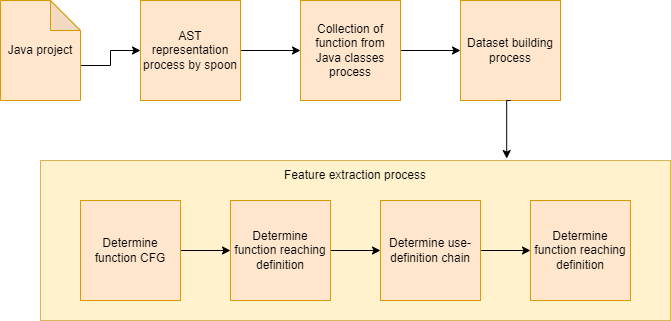
\includegraphics[width=0.95\textwidth]{TransformationProcess2}
	  \caption{Java project transformation process}
  \label{fig:transfProcess}
\end{figure}

To create the dataset, there are dependencies between different processes, as shown in the Figure \ref{fig:transfProcess}. The representation of the source codes was transformed into \gls{ast} and then \gls{cfg} to facilitate static analysis of the source code. With the use-definition chain, it is possible to determine which variables are being used in the invocation of each function. These functions and their respective argument values are extracted to build the dataset. Figure \ref{fig:DattDesc} represents the description of the dataset.

\begin{figure}[ht]
	\centering
	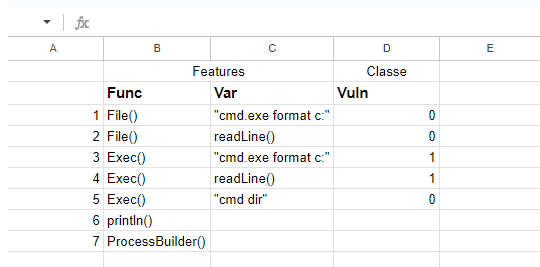
\includegraphics[width=0.95\textwidth]{DatasetDescription}
	  \caption{Dataset description}
  \label{fig:DattDesc}
\end{figure}

The attribute "Func" represents potentially vulnerable invoked methods.
The attribute "Var" represents the values of the arguments passed to the methods.
The attribute "Vuln" represents the class of the dataset. It indicates whether a row is vulnerable or not.

The attributes "Func" and "Var" represent characteristics of our problem, serving as inputs to the model. The attribute "Vuln" represents the model's output, indicating whether a row is vulnerable or not.

The model learns whether the functions are vulnerable or not based on the values of the arguments that are passed to these functions. The dataset has been saved in a Comma-separated values (CSV) file.


% section Data_Tranformation (end)

\section{Model Creation} % (fold)
\label{sec:	Model_Creation}

This section corresponds to the second phase of the proposed architecture.

Once we have the dataset created and ready to be used in training, we are able to create the model. This section describes the entire implementation process.

Figure \ref{fig:model_creation_methodology} illustrates the actions carried out in the model creation process. Next, we will describe these steps.

\begin{figure}[ht]	
	\centering
	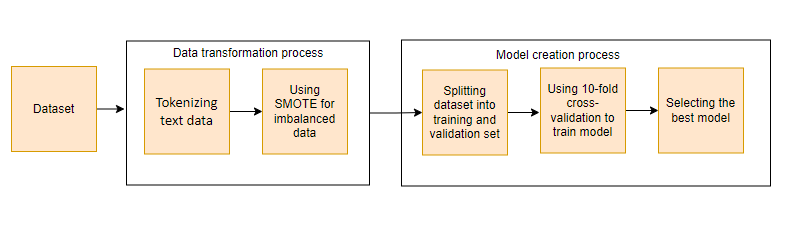
\includegraphics[width=0.95\textwidth]{OverviewModelCreation}
	  \caption{Overview of the methodology used to create the model.}
  \label{fig:model_creation_methodology}
\end{figure}

\begin{enumerate}
\item \textbf{Tokenizing text data}

In order to perform machine learning on text data, we first need to transform text content into numerical feature vectors \cite{Text_Data}. Since we are using text data, it requires special preparation before we can start using it for predictive modeling. 

The text must be parsed to isolate words, in a process called \textit{tokenization}. Then the words need to be encoded as integers or floating point values for use as input to a machine learning algorithm,  a process known as \textit{vectorization}.

This can be done by assigning to each word a unique number. Any text in our data can be encoded as a fixed-length vector with the length of the vocabulary of known words. The value in each position in the vector could be filled with a count or frequency of each word in the encoded document.

This is the bag of words model \cite{Text_Data}, where we are only concerned with encoding schemes that represent what words are present or the degree to which they are present in encoded documents without any information about order.

We used the scikit-learn library tools to perform tokenization of text data \cite{scikit_learn_Text_Data}.

\item \textbf{Using Synthetic Minority Oversampling Technique (SMOTE) for imbalanced classification data}

Given that in our dataset the distribution of classes is significantly skewed, the class "not vulnerable" (the minority class) has a much smaller number of samples compared to the "vulnerable" class (the majority class) \cite{SMOTE_Jason}.

Our model's training data has been biased towards the majority class, making it challenging for the model to accurately predict the minority class. As a result, the classification algorithms have been biased in favor of the majority class, leading to poor performance for the minority class.

To solve this problem, we were forced to oversample the examples in the minority class (vulnerable class). This have been achieved by simply duplicating examples from the minority class in the dataset prior to fitting a model. This was able to balance the class distribution without providing any additional information to the model.

 The improvement on duplicating examples from the minority class is to synthesize new examples from the minority class. This is a type of data augmentation for tabular data and can be very effective.

 We used the most common and widely approach to synthesizing new examples called the \gls{smote}. This technique is described by Nitesh Chawla, et al. in \cite{chawla2002smote}.

 \gls{smote} works by selecting examples that are close in the feature space, drawing a line between the examples in the feature space and drawing a new sample at a point along that line \cite{SMOTE_Jason}.

In our python project, we used the implementations provided by the imbalanced-learn Python library \cite{imbalanced_scikit}, which we installed via pip.


\item \textbf{Splitting dataset into training and validation set}

After parsing our text data into numerical feature vectors and then applying SMOTE to balance our class, the next step was to split the dataset into the following subsets:

\textbf{Training Set} was used to train the machine learning model. The model learns from the patterns and features present in the training data to make predictions on new, unseen data.

\textbf{Validation Set} was used to evaluate the performance of the trained model. It serves as a proxy for new, unseen data and helps assess how well the model generalizes to unseen examples.


The purpose of splitting the dataset was to avoid \textit{overfitting}, where the model performs well on the data it was trained on but poorly on new data. By having a separate validation set, you can assess the model's performance on unseen data and choose the best parameters for the model to achieve better generalization.

The dataset was randomly divided into the training and validation sets, with the split ratio 60\% for training and 40\% for validation.

\item \textbf{Using K-fold cross-validation}

Is a common technique used to assess the performance of a model. It involves dividing the dataset into k equal parts (folds) and then training and evaluating the model k times. In each iteration, one fold is used as the test set, and the remaining nine folds are used as the training set. This process is repeated ten times, ensuring that each fold is used as the test set once. The results of the ten evaluations are then averaged to obtain a more robust and reliable performance estimate for the model \cite{inbook_Cross_Validation}.

The main reason for using k-fold cross-validation was because it is easy to understand, implement, and generally results in less biased estimates (less optimistic estimation of the model) compared to other methods. It also allows the random division of data.

Sampling bias is a systematic error due to a non-random sample of a population, causing some members of the population to be less likely to be included than others, resulting in a biased sample \cite{inbook_Cross_Validation}.

The procedure has a parameter called k, which refers to the number of groups to which each data sample should be divided. Then, the average of the result is calculated for each instance (group).

The procedure is as follows:
\begin{itemize}
    \item Randomly divide the data into K-folds (K groups). The higher the value of K, the less biased the model.
    \item Fit the model using the first K-1 groups of data and validate the model using the remaining K group of data.
    \item Repeat the procedure until each K-fold (each group) serves as the test dataset. Then, take the resulting average of each instance. This is the performance metric for the model.
\end{itemize}

There are 2 variations of cross-validation commonly used: Stratified and Repeated, both available in scikit-learn \cite{ros_validation_scikit}.

\textbf{Stratified}: The division of data into groups can be more strict. It may have criteria such as ensuring that each group has the same proportion of observations with a certain categorical value, such as the class outcome value.
Meaning that each group or data division will have the same distribution of examples per class existing in the entire training dataset.

\textbf{Repeated}: The validation procedure is repeated n times. The crucial aspect is that the data sample is shuffled before each repetition, resulting in a different split of the sample.

We had used stratified 10-fold cross-validation to estimate model accuracy.  This had split our dataset into 10 parts, trained on 9, and tested on 1, and repeated for all combinations of train-test splits. We used the metric of 'accuracy' to evaluate models. This is a ratio of the number of correctly predicted instances divided by the total number of instances in the dataset multiplied by 100 to give a percentage (e.g., 95\% accurate). We used the scoring variable to build and evaluate each model.

\newpage

\item \textbf{Build multiple different models to predict vulnerability from our dataset}

Since we didn't know which algorithms would be good for our problem or what configurations to use, we had to create different models using various algorithms.

We used a mixture of simple linear, with nonlinear algorithms. We decided to also use deep learning (Multi-layer Perceptron classifier) to make a small experiment. The followings algorithms were used on the process:
\begin{itemize}
    \item \gls{lr}
    \item \gls{dt}
    \item \gls{nc}
    \item \gls{nb}
    \item Support Vector Machine (SVM)
    \item \gls{mlpc} - Deep Learning.
\end{itemize}

\item \textbf{Select the best model as our final model}

After building and evaluating different models, we compared the models to each other and selected the most accurate one as our final model.

Afterward, we used the validation set to understand the accuracy of the final model. We fitted the final model on the entire training dataset and made predictions on the validation dataset. We evaluated the predictions by comparing them to the expected results in the validation set, then we calculated the classification accuracy, as well as a confusion matrix and a classification report. All the experimental results are described in the Chapter \ref{cha:Evaluation_chapter}.
\end{enumerate}

% section Model_Creation (end)